\documentclass[11pt]{article}
\usepackage[a4paper,margin=28mm]{geometry}
\usepackage[T1]{fontenc}
\usepackage{lmodern,microtype,amsmath,amssymb,amsthm,mathtools}
\usepackage{booktabs,array,enumitem,xcolor,tikz}
\usepackage[colorlinks=true,linkcolor=blue!45!black,citecolor=blue!45!black,urlcolor=blue!45!black]{hyperref}
\hypersetup{pdftitle={Arithmetic Rank and Differential Complexity of Hamiltonian Moment Integrals},pdfauthor={KEIO}}
\newtheorem{theorem}{Theorem}[section]
\newtheorem{lemma}[theorem]{Lemma}
\newtheorem{proposition}[theorem]{Proposition}
\newtheorem{corollary}[theorem]{Corollary}
\theoremstyle{definition}
\newtheorem{definition}[theorem]{Definition}
\newtheorem{example}[theorem]{Example}
\theoremstyle{remark}
\newtheorem{remark}[theorem]{Remark}
\newcommand{\R}{\mathbb R}
\newcommand{\Q}{\mathbb Q}
\newcommand{\C}{\mathbb C}
\newcommand{\Z}{\mathbb Z}
\newcommand{\N}{\mathbb N}
\newcommand{\dd}{\,d}
\DeclareMathOperator{\supp}{supp}
\DeclareMathOperator{\ord}{ord}
\DeclareMathOperator{\spanQ}{span_{\mathbb Q}}
\newcommand{\CP}{\mathbb {CP}}
\setlength{\emergencystretch}{2em}
\setlist{leftmargin=*,itemsep=3pt}
\numberwithin{equation}{section}
\title{Arithmetic Rank and Differential Complexity\\of Hamiltonian Moment Integrals}
\author{KEIO}
\date{20 October 2026}
\begin{document}
\maketitle
\begin{abstract}
For the diagonal Hamiltonian circle action on a product of $n$ symplectic
two-spheres, we determine the scalar differential complexity of the
exponential moment integral after all collisions of fixed-point values
have been combined. If the moment lengths have rational rank $r$, the
minimal differential order is at least $2^{r-1}(n-r+2)$. This bound is
attained for every $1\le r\le n$. The combinatorial input is a sharp
support bound for a product of $n$ Laurent binomials spanning rank $r$,
proved by counting vertices and edge-interior coefficients of its Newton
zonotope. We also give an exact formula when the rational relation space
is one-dimensional. For the uncentered Hamiltonian moments, we classify
every polynomial-coefficient recurrence: its order is at least one less
than the surviving exponential support, and each coefficient has a
specified degree-$n$ divisor. The differential Galois group is a torus
of dimension $r$. These results distinguish the number of fixed points,
the number of critical levels, and the number of analytically visible
levels. The localization and spline formulas are classical; the paper
supplies complete proofs of the support and complexity statements and
does not claim a resolution of a named open conjecture.
\end{abstract}
\noindent\textbf{Keywords.} Hamiltonian circle action; Duistermaat--Heckman
measure; zonotope; sparse polynomial; rational rank; differential equation;
polynomial recurrence.

\section{The problem and the main result}
The exponential integral of a Hamiltonian moment map is constrained by
the fixed points of the action. What is less immediate is how many of
those constraints survive when several fixed points have the same moment
value. An upper differential equation obtained by multiplying all
fixed-point factors can substantially overestimate the minimum order.
We investigate that loss of complexity for products of symplectic spheres.

Let $a=(a_1,\ldots,a_n)$ with $a_i>0$, and define
\begin{equation}\label{eq:main-F}
 F_a(t)=\prod_{i=1}^n\frac{e^{a_i t}-1}{a_i t},\qquad F_a(0)=1.
\end{equation}
Section~\ref{sec:geometry} realizes this function as a normalized
symplectic integral. For a subset $S\subseteq[n]$, write
$a(S)=\sum_{i\in S}a_i$. Set
\begin{equation}\label{eq:visible-def}
\begin{aligned}
 c_\lambda&=\sum_{S:\,a(S)=\lambda}(-1)^{n-|S|},
 &\Sigma_a&=\{\lambda:c_\lambda\ne0\},\\
 N(a)&=|\Sigma_a|,
 &r(a)&=\dim_\Q\spanQ\{a_1,\ldots,a_n\}.
\end{aligned}
\end{equation}
Thus $0$ and $A=\sum_i a_i$ belong to $\Sigma_a$. All its other
elements are positive and smaller than $A$. Define $\operatorname{dord}F$
as the least order of a nonzero scalar linear differential operator over
$\C(t)$ annihilating $F$.

\begin{theorem}[Arithmetic rank and differential complexity]
\label{thm:main}
For every positive tuple $a$,
\begin{equation}\label{eq:main-bound}
 \operatorname{dord}F_a=N(a)\ge
 2^{r(a)-1}\bigl(n-r(a)+2\bigr).
\end{equation}
For every pair $1\le r\le n$, positive lengths of rational rank $r$
attain equality. In particular, rationally independent lengths give
order $2^n$, and order $n+1$ forces all lengths to be commensurable
when $n\ge2$.

Writing $F_a(t)=\sum_{k\ge0}m_k t^k/k!$, the minimum order of a
polynomial-coefficient recurrence for $(m_k)$ is $N(a)-1$, and the
minimum coefficient degree among all such recurrences is $n$.
The differential Galois group of the minimal differential equation
over $\C(t)$ is an algebraic torus of dimension $r(a)$.
\end{theorem}

Here commensurable means that every ratio $a_i/a_j$ is rational. The
converse to the order-$n+1$ assertion is false: for example, lengths
$(1,2)$ are commensurable but yield four exponential terms. The
recurrence statement uses the normalization $\min H=0$; shifting a
Hamiltonian preserves differential order but can change recurrence order.

\subsection{Proof dependencies and relation to earlier work}
The analytic transfer used here is specific. The grouped local-connection
formula for weighted Jacobi pushforwards in \cite[Part IX, theorem
``Weighted graphical Jacobi local connections'']{KeioUnified} specializes
to the present setting by taking every endpoint exponent and interaction
exponent to be zero, the analytic amplitude to be one, and the linear
weights to be $a_i$. Equal subset sums must then be combined with their
signs. The dual-singular-support lemma of \cite[Section 3.1]{KeioVertex}
turns each surviving non-smooth level into a lower bound on differential
order. Its negative-exponent transfer principle motivates the recurrence
divisibility statement below. We reproduce these specializations and
their proofs; no unverified classification from either manuscript is
needed as a black box.

The additional ingredient is geometric: a Newton zonotope and its
central hyperplane arrangement force enough coefficients to survive,
even when subset sums collide. It is this step that produces the
rational-rank bound, which does not follow merely by counting fixed
points. The exact corank-one formula separately identifies which single
rational relations produce cancellation.

Duistermaat--Heckman localization and its equivariant formulation are
classical \cite{DH,AB}. In the product model, they reduce to integration
over intervals; the resulting density is a univariate box spline
\cite{BoxSplines}. The binomial products themselves belong to the
established literature on pure products, root systems, and discrete
tomography \cite{MaltbyPTE,MaltbyRoots,AlpersLarman}. We do not present
those connections, the spline formula, or exponential independence as
new. A focused literature comparison did not establish historical
priority for the combined sharp rank-and-complexity statement. This
manuscript records a self-contained theorem and proof, not a certified
priority or publication-level assessment.

\section{The Hamiltonian model and visible critical levels}
\label{sec:geometry}
Equip each sphere $S^2_i\simeq\CP^1$ with a rotationally invariant
symplectic form and the standard rotation action. Normalize the angular
coordinate to have period one and the moment coordinate $x_i$ to range
over $[0,a_i]$. On the complement of the poles, the symplectic form is
$dx_i\wedge d\theta_i$. Consequently its pushforward under $x_i$ is
Lebesgue measure on $[0,a_i]$. On
\[
 M_a=(S^2)^n,\qquad \omega_a=\sum_i\pi_i^*\omega_i,
\]
the diagonal circle action has moment map $H_a=\sum_i x_i$ and $2^n$
isolated fixed points. Its normalized Liouville measure pushes forward
to the convolution of the uniform probability measures on $[0,a_i]$.
This proves \eqref{eq:main-F} directly. The endpoint lengths may be
arbitrary positive real numbers; an integral symplectic class is not
assumed.

\begin{proposition}[Exact collision and visibility formula]
\label{prop:spline}
Put $V=\prod_i a_i$. The pushforward density satisfies, as a distribution,
\begin{equation}\label{eq:spline}
 \rho_a(x)=\frac{1}{V(n-1)!}
   \sum_{S\subseteq[n]}(-1)^{|S|}(x-a(S))_+^{n-1},
\end{equation}
with $x_+^0=\mathbf1_{x>0}$ when $n=1$. In particular,
\begin{equation}\label{eq:delta-jumps}
 D_x^n\rho_a=\frac{(-1)^n}{V}
          \sum_{\lambda\in\Sigma_a}c_\lambda\delta_\lambda.
\end{equation}
The density is polynomial on each component of $\R\setminus\Sigma_a$.
At each $\lambda\in\Sigma_a$, its $(n-1)$st derivative has a nonzero
jump. At a subset sum with $c_\lambda=0$, it is polynomial across that
level. Thus $\Sigma_a$ is exactly its non-smooth locus.
\end{proposition}
\begin{proof}
For one interval, $D\mathbf1_{[0,a_i]}=\delta_0-\delta_{a_i}$.
Differentiate the convolution once in each factor to obtain
$D^n\rho_a=V^{-1}\mathop{*}_{i=1}^n(\delta_0-\delta_{a_i})$.
The distribution $(x-b)_+^{n-1}/(n-1)!$ is the unique $n$th primitive
of $\delta_b$ vanishing on the far left, giving \eqref{eq:spline}.
Grouping equal subset sums gives \eqref{eq:delta-jumps}. The local
polynomial and jump assertions follow immediately.
\end{proof}

\begin{lemma}[Dual singular support]\label{lem:dual-local}
Let $\rho$ be a compactly supported distribution and
$F(t)=\langle\rho,e^{tx}\rangle$. If
$L=\sum_{j=0}^q p_j(t)\partial_t^j\ne0$ has polynomial coefficients
and $LF=0$, set $d=\max_j\deg p_j$ and
$\chi_L(x)=\sum_j[t^d]p_j(t)x^j$. Then $\rho$ is real analytic
away from the zeros of the nonzero polynomial $\chi_L$, whose degree
is at most $q$.
\end{lemma}
\begin{proof}
Fourier--Laplace injectivity gives
$\widehat L\rho=0$, where
$\widehat L=\sum_j p_j(-D_x)\circ x^j$.
Its highest derivative coefficient is $(-1)^d\chi_L(x)$.
If $d=0$, this says $\chi_L\rho=0$. If $d>0$, away from its zeros
the distributional equation is an ordinary analytic first-order system
for $(\rho,D\rho,\ldots,D^{d-1}\rho)$. Multiplying by the inverse of
an analytic fundamental matrix shows that this vector is an analytic
matrix times a constant vector. Hence $\rho$ is analytic there.
\end{proof}

\begin{proposition}[Minimum scalar order]\label{prop:min-order}
Let $P_a(z)=\prod_{\lambda\in\Sigma_a}(z-\lambda)$.
The monic minimal operator of $F_a$ over $\C(t)$ is
\begin{equation}\label{eq:min-operator}
 L_a=t^{-n}P_a(\partial_t)\,t^n.
\end{equation}
It has order $N(a)$ and no finite singularity outside zero.
\end{proposition}
\begin{proof}
Since $Vt^nF_a=\sum_\lambda c_\lambda e^{\lambda t}$, the displayed
operator annihilates $F_a$ and has order $N(a)$. Conversely,
Proposition~\ref{prop:spline} and Lemma~\ref{lem:dual-local} force the
top-degree polynomial of every polynomial annihilator to vanish at all
$N(a)$ visible levels. Its order is at least $N(a)$. Clearing rational
denominators does not change order. The displayed monic operator must
therefore be minimal; its coefficients have poles only at zero.
\end{proof}

The lower bound just proved is the actual use of the earlier visibility
method. Formula \eqref{eq:spline} is its collision-sensitive input.
Counting the $2^n$ fixed points without grouping would give a false
answer, as the examples below show.


\section{A sharp support bound for products of binomial differences}
\label{sec:support-rank}

The following argument is independent of symplectic localization. All
coefficients are taken in a field of characteristic zero.

\begin{theorem}\label{thm:binomial-rank}
Let $v_1,\ldots,v_n\in\mathbb Z^r\setminus\{0\}$ span
$\mathbb R^r$, and put
\[
 B(X)=\prod_{i=1}^n(1-X^{v_i})
       \in\mathbb C[X_1^{\pm1},\ldots,X_r^{\pm1}].
\]
Then
\[
 |\operatorname{supp}B|\ge 2^{r-1}(n-r+2).
\]
This bound is attained for every $1\le r\le n$.
\end{theorem}

\begin{proof}
Partition the vectors into $k$ parallel classes, of respective sizes
$m_1,\ldots,m_k$, so that $\sum_jm_j=n$. The Newton polytope of $B$ is
the full-dimensional zonotope
\[
 Z=\sum_{i=1}^n[0,v_i].
\]
The identity follows either from the usual product rule for Newton
polytopes or directly by exposing a vertex with a generic linear
functional: in each binomial the exposed endpoint is unique, so the
coefficient of the exposed vertex cannot cancel.

We first count vertices. This is the standard central-arrangement
minimum-region argument; see also the extremal-arrangement literature
\cite{Zaslavsky}. Let $H_j$ be the hyperplane orthogonal to the
$j$th parallel class. The vertices of $Z$ correspond to the chambers of
the central arrangement $\{H_1,\ldots,H_k\}$. Start with $r$ hyperplanes
whose normals are independent. These have $2^r$ chambers. Adding a
further distinct hyperplane $H$ increases the number of chambers by the
number of chambers of the arrangement induced on $H$. The induced
arrangement is essential in $H$: the restrictions to $H$ of the original
$r$ independent normal forms span $H^*$. It therefore has at least
$2^{r-1}$ chambers. Consequently the number $V$ of vertices satisfies
\[
 V\ge 2^r+(k-r)2^{r-1}
   =2^{r-1}(k-r+2).
\]
For $r=1$ there is just one parallel class and $V=2$, consistent with
the same formula.

For each class $j$, a functional in $H_j$ avoiding all the other
hyperplanes exposes an edge parallel to that class. The resulting
edges are indexed by the chambers of the induced arrangement on $H_j$.
Thus the number $E_j$ of these edges is at least $2^{r-1}$. In dimension
one, take the segment $Z$ itself as its unique edge, so that $E_1=1$.

On any such edge, the face polynomial of $B$ is a Laurent monomial times
the product of precisely the $m_j$ binomials from the $j$th class.
Writing the class vectors as nonzero integer multiples of a primitive
lattice vector identifies this product, up to a Laurent monomial, with
\[
 \prod_{i=1}^{m_j}(1-z^{q_i}),\qquad q_i\in\mathbb Z\setminus\{0\}.
\]
It has a zero of exact order $m_j$ at $z=1$. A nonzero Laurent
polynomial with $s$ nonzero terms has vanishing order at most $s-1$
there: applying $(z\partial_z)^a$ for $a=0,\ldots,s-1$ gives an
invertible Vandermonde matrix in its distinct exponents. The face
polynomial therefore has at least $m_j+1$ terms. Its two extreme terms
are the edge endpoints, leaving at least $m_j-1$ support points in the
relative interior of the edge.

Distinct edges have disjoint relative interiors. Counting vertices and
these edge-interior support points gives
\begin{align*}
 |\operatorname{supp}B|
 &\ge V+\sum_{j=1}^kE_j(m_j-1)\\
 &\ge 2^{r-1}(k-r+2)+2^{r-1}(n-k)
  =2^{r-1}(n-r+2).
\end{align*}
Finally, choose $n-r+1$ copies of $e_1$, and one copy of each of
$e_2,\ldots,e_r$. The resulting polynomial is
$(1-X_1)^{n-r+1}\prod_{j=2}^r(1-X_j)$, whose support has exactly
$(n-r+2)2^{r-1}$ elements.
\end{proof}

\begin{corollary}\label{cor:real-length-rank}
Let $a_1,\ldots,a_n>0$, let
$r=\dim_{\mathbb Q}\operatorname{span}_{\mathbb Q}\{a_1,\ldots,a_n\}$,
and combine equal exponents in
$\prod_i(e^{a_it}-1)=\sum_{s\in\Sigma}c_s e^{st}$, with every
$c_s\ne0$. Then
\[
 |\Sigma|\ge2^{r-1}(n-r+2).
\]
In particular, $|\Sigma|=n+1$ forces $r=1$ when $n\ge2$.
\end{corollary}

\begin{proof}
Choose a rational basis for the lengths and clear all denominators to
write $a_i=\langle v_i,b\rangle$ with $v_i\in\mathbb Z^r$ and the
coordinates of $b$ linearly independent over $\mathbb Q$. Distinct
integer exponent vectors then give distinct real exponents, so the
preceding theorem applies without loss of support. For $r\ge2$, its
bound is at least $2n>n+1$; indeed
$2^{r-1}(n-r+2)\ge2n$ for $n\ge r\ge2$.
\end{proof}

\begin{proposition}[Three positive lengths]\label{prop:three-lengths}
For three positive lengths, $|\Sigma|=4$ if and only if, up to
permutation and common scale, their multiset is $(1,1,1)$ or $(1,1,2)$.
\end{proposition}

\begin{proof}
Write $a\le b\le c$ and $A=a+b+c$. If $a<b$, the coefficients at
$a$ and $b$ in $\prod(e^{a_it}-1)$ are both nonzero: no pair of the
three lengths can sum to either value. Their reflected exponents
$A-a$ and $A-b$ are also nonzero, by antisymmetry about $A/2$.
These four exponents are distinct and lie strictly between $0$ and
$A$, yielding at least six support points. Thus $a=b$ is necessary.
For $(a,a,c)$ the candidate exponents are
$0,a,2a,c,c+a,c+2a$. If $c>a$ and $c\ne2a$ they are all distinct,
so there are six terms. If $c=a$, expansion gives four terms, and if
$c=2a$ the terms at $2a$ cancel, again leaving four.
\end{proof}



\section{Exact collisions in rational corank one}
\label{sec:corank-one}

The sharp support bound admits a complete refinement when there is only
one rational relation among the parameters. This refinement distinguishes
three phenomena: a rational dependence can produce no subset-sum
collision; a collision can merge two coefficients without cancellation;
or it can cancel both coefficients.

For a tuple $a=(a_1,\ldots,a_n)$ of positive real numbers, write
\[
 G_a(t)=\prod_{i=1}^n(e^{a_i t}-1)
       =\sum_{\lambda}c_\lambda e^{\lambda t},
 \qquad
 N(a)=\#\{\lambda:c_\lambda\ne0\},
\]
where equal exponents have been collected before $N(a)$ is counted.
The integral relation lattice is
\[
 \mathcal R(a)=
 \left\{u\in\mathbb Z^n:\sum_{i=1}^n u_i a_i=0\right\}.
\]
If $\dim_{\mathbb Q}\operatorname{span}_{\mathbb Q}\{a_i\}=n-1$,
then $\mathcal R(a)=\mathbb Z u$ for a primitive integer vector $u$,
unique up to sign. Here primitive means that the greatest common divisor
of its coordinates is one.

\begin{theorem}[Exact support in rational corank one]
\label{thm:corank-one}
Let $n\ge2$ and let $a_1,\ldots,a_n>0$ have rational rank $n-1$.
Let $u$ be a primitive generator of $\mathcal R(a)$.
\begin{enumerate}
\item If $|u_i|>1$ for some $i$, then every subset sum of the $a_i$ is
distinct and
\[
 N(a)=2^n.
\]
\item Otherwise, every nonzero coordinate of $u$ belongs to
$\{-1,1\}$. Put $c=\#\{i:u_i\ne0\}$. Then $c\ge2$ and
\begin{equation}
\label{eq:corank-one-support}
 N(a)=
 \begin{cases}
  2^n-2^{n-c},&c\text{ even},\\
  2^n-2^{n-c+1},&c\text{ odd}.
 \end{cases}
\end{equation}
\end{enumerate}
Consequently,
\begin{equation}
\label{eq:corank-one-minimum}
 N(a)\ge3\cdot2^{n-2},
\end{equation}
with equality if and only if, after permuting coordinates and changing
the sign of $u$, the unique rational relation is of one of the forms
\[
 a_1=a_2,
 \qquad\text{or}\qquad
 a_1+a_2=a_3.
\]
The second possibility requires $n\ge3$. In both cases the statement
that the relation is unique is part of the hypothesis: all remaining
parameters are independent modulo that relation.
\end{theorem}

\begin{proof}
For a subset $S\subseteq\{1,\ldots,n\}$ let
$\mathbf1_S\in\{0,1\}^n$ be its indicator vector and put
$a(S)=\sum_{i\in S}a_i$. If $a(S)=a(T)$, then
\[
 \mathbf1_S-\mathbf1_T\in\mathcal R(a)=\mathbb Z u.
\]
For completeness, the multiplier is an integer, not merely rational:
if $q u\in\mathbb Z^n$ and $u$ is primitive, a Bezout combination of
the coordinates of $u$ shows that $q\in\mathbb Z$.

Every coordinate of $\mathbf1_S-\mathbf1_T$ lies in $\{-1,0,1\}$.
If some $|u_i|>1$, no nonzero multiple of $u$ can have this property.
Thus $S=T$ in every collision, proving the first assertion.

Assume now that the nonzero coordinates of $u$ are all $\pm1$, and
set
\[
 A=\{i:u_i=1\},\qquad B=\{i:u_i=-1\},\qquad
 C=\{1,\ldots,n\}\setminus(A\cup B).
\]
The positivity of the $a_i$ ensures that $A$ and $B$ are both nonempty.
The relation is $a(A)=a(B)$ and $c=|A|+|B|\ge2$.

If two distinct subsets have equal sums, their indicator difference is
$u$ or $-u$: larger integer multiples are impossible inside the binary
cube. After exchanging the subsets if necessary, they must therefore be
\begin{equation}
\label{eq:corank-one-pairs}
 A\cup T\quad\text{and}\quad B\cup T,
 \qquad T\subseteq C.
\end{equation}
Conversely, every pair in \eqref{eq:corank-one-pairs} has equal sums.
There are exactly $2^{n-c}$ such pairs. Their common sums are distinct
from one another and from all other subset sums. Indeed, every fiber
of the subset-sum map has at most two elements: three distinct elements
on an affine line with direction $u$ would include two whose difference
has a coordinate of absolute value at least two.

The contribution of a subset $S$ to $G_a$ is
$(-1)^{n-|S|}e^{a(S)t}$. For the two subsets in
\eqref{eq:corank-one-pairs}, the ratio of the signs is
$(-1)^{|A|-|B|}=(-1)^c$. When $c$ is even, the two equal exponents
merge into one term with a nonzero coefficient. Each pair therefore
decreases the support count by one. When $c$ is odd, the coefficients
cancel and each pair decreases the support count by two. This proves
\eqref{eq:corank-one-support}.

If $c$ is even, then $c\ge2$ and the deficit from $2^n$ is at most
$2^{n-2}$, with equality precisely when $c=2$. If $c$ is odd, then
$c\ge3$ and the deficit is again at most $2^{n-2}$, with equality
precisely when $c=3$. Positivity turns the corresponding primitive
relations into $a_i=a_j$ and $a_i+a_j=a_k$, respectively. The case
with a coordinate $|u_i|>1$ has support $2^n$ and is never extremal.
\end{proof}

\begin{example}
Let $a,b>0$ be rationally independent. The tuple $(a,b,a+b)$ has
six surviving exponents: its one collision cancels the two terms at
$a+b$. The tuple $(a,b,2a+b)$ has the same rational rank but all eight
subset sums are distinct. Rational dependence alone therefore does not
imply a loss of exponential support.

For three positive rationally independent numbers $a,b,c$, the tuple
$(a,b,c,a+b)$ attains the corank-one minimum $12$. In contrast,
$(a,b,c,a+b+c)$ has support $15$: its unique colliding pair has equal
signs and merges rather than cancels.
\end{example}


\section{All polynomial recurrences and their unavoidable factors}
\label{sec:symplectic}

We first establish the scalar statement needed for the geometric
application. Write $D=d/dt$ and
\[
 h_n(k)=(k+1)(k+2)\cdots(k+n).
\]
A polynomial recurrence has the form $\sum_{j=0}^M p_j(k)m_{k+j}=0$
for all sufficiently large integers $k$, with $p_0p_M\ne0$. Its
order is $M$ and its coefficient degree is $\max_j\deg p_j$.

\begin{theorem}[Exponential numerator and all polynomial recurrences]
\label{thm:exponential-numerator}
Let $n\ge1$, let
$0=\lambda_0<\lambda_1<\cdots<\lambda_s$, and let all
$c_0,\ldots,c_s$ be nonzero real numbers. Suppose
\[
 G(t)=\sum_{i=0}^s c_i e^{\lambda_i t}
\]
has a zero of exact order $n$ at $0$. Put $F(t)=t^{-n}G(t)$ and
$m_k=F^{(k)}(0)$. Define
\[
 P(z)=\prod_{i=0}^s(z-\lambda_i),\qquad
 Q(z)=\prod_{i=1}^s(z-\lambda_i)=\sum_{j=0}^s q_jz^j.
\]
Then the following assertions hold.
\begin{enumerate}
\item $s\ge n$. The minimal order over $\mathbb C(t)$ of a nonzero
linear differential operator annihilating $F$ is $s+1$. Its monic
minimal operator is
\[
 L=t^{-n}\circ P(D)\circ t^n.
\]
The polynomial-coefficient operator
$L_{\rm pol}=P(D)\circ t^n$ is primitive, has leading coefficient
$t^n$, and has no finite singularity except possibly $0$.
\item The indicial roots of $L$ at $0$ are
\[
 -n,-n+1,\ldots,s-n.
\]
Writing $\theta=tD$, the operator
$t^{s+1-n}L_{\rm pol}$ has $\theta$-span $s$, with lowest
$\theta$-coefficient $(\theta+n)^{\underline{s+1}}$.
\item The moments satisfy
\[
 \sum_{j=0}^s q_j h_n(k+j)m_{k+j}=0\qquad(k\ge0).
\]
This recurrence has minimal order $s$ and minimal coefficient degree
$n$ among all eventual polynomial-coefficient recurrences.
\item More precisely, for arbitrary $M\ge0$ and
$p_0,\ldots,p_M\in\mathbb C[k]$, the identity
\[
 \sum_{j=0}^M p_j(k)m_{k+j}=0
\]
holds for all sufficiently large integers $k$ if and only if
\[
 h_n(k+j)\mid p_j(k)\quad(0\le j\le M),\qquad
 Q(z)\mid\sum_{j=0}^M\frac{p_j(k)}{h_n(k+j)}z^j
       \quad\hbox{in }\mathbb C[k,z].
\]
Consequently every recurrence of order $s$ is a polynomial in $k$
times the displayed recurrence, and its degree-$n$ representative is
unique up to a nonzero constant.
\end{enumerate}
\end{theorem}

\begin{proof}
The $s+1$ by $s+1$ Vandermonde matrix in the distinct $\lambda_i$
shows that a nonzero sum of these exponentials cannot have a zero of
order greater than $s$. Hence $s\ge n$.

Distinct real exponentials are linearly independent over
$\mathbb C(t)$. Indeed, in any nontrivial relation, a nonzero rational
coefficient of the largest exponential behaves as a nonzero constant
times a power of $t$ as $t\to+\infty$, whereas all terms of smaller
exponential rate decay exponentially after division by that largest
exponential. This is impossible. If an operator
$A=\sum_{j=0}^m a_j(t)D^j$ annihilates $G$, this independence implies
$\sum_j a_j(t)\lambda_i^j=0$ for every $i$. When $m<s+1$, a
polynomial of degree at most $m$ cannot vanish at all $s+1$ distinct
$\lambda_i$, unless all $a_j$ vanish. Thus $P(D)$ is the monic
minimal operator of $G$, and rational gauge conjugation proves the
assertion for $F$.

The leading coefficient of $P(D)\circ t^n$ is $t^n$.
The coefficient of $D^{s+1-n}$ has nonzero constant term
$\binom{s+1}{n}n!$, arising from the leading term of $P(D)$;
lower-degree terms of $P$ contribute only positive powers of $t$ to
that coefficient. Thus no factor of $t$ divides every coefficient,
and primitivity follows. If $P(z)=\sum_{j=0}^{s+1}b_jz^j$, then
\[
 t^{s+1-n}L_{\rm pol}
 =\sum_{j=0}^{s+1}b_jt^{s+1-j}
             (\theta+n)^{\underline j}.
\]
Here $b_0=0$, $b_1\ne0$, and $b_{s+1}=1$. This proves the span and
indicial assertions. It also proves regular singularity at $0$.

Coefficient extraction gives
\[
 m_k=\frac{k!}{(k+n)!}\sum_{i=0}^s c_i\lambda_i^{k+n}
     =\frac1{h_n(k)}\sum_{i=1}^s d_i\lambda_i^k,
 \qquad d_i=c_i\lambda_i^n\ne0.
\]
The zero phase disappears because $k+n>0$. Consequently
$b_k=h_n(k)m_k$ is annihilated by the constant-coefficient shift
operator $Q(E)$, where $(Eb)_k=b_{k+1}$. This gives the claimed
recurrence.

It remains to prove the classification, including its saturation at
every negative integer pole. Suppose an eventual recurrence holds.
The sequences $\lambda_i^k$ are linearly independent over
$\mathbb C(k)$, by the same largest-rate argument along positive
integers. Therefore, for every $i=1,\ldots,s$,
\[
 R_i(k):=\sum_{j=0}^M
        \frac{p_j(k)}{h_n(k+j)}\lambda_i^j=0
        \quad\hbox{in }\mathbb C(k).
\]
Fix an integer $\ell$. The terms with a possible pole at $k=-\ell$
are precisely the shifts
\[
 j\in J_\ell=[\ell-n,\ell-1]\cap[0,M]\cap\mathbb Z.
\]
All these poles are simple and $J_\ell$ contains at most $n$
consecutive integers. Taking residues in the identities $R_i=0$
gives a polynomial in $z$ of the form
\[
 A_\ell(z)=\sum_{j\in J_\ell}r_jz^j
\]
which vanishes at all $s$ nonzero numbers $\lambda_i$. After removing
its smallest possible power of $z$, its degree is at most $n-1<s$.
It is therefore identically zero. Every residue $r_j$ vanishes.
For a fixed shift $j$, varying $\ell=j+1,\ldots,j+n$ proves that
$p_j$ vanishes at every root of $h_n(k+j)$, so that
$h_n(k+j)\mid p_j(k)$.

The resulting polynomial
$A(k,z)=\sum_j[p_j(k)/h_n(k+j)]z^j$ vanishes at every $\lambda_i$.
Division by the monic constant-coefficient polynomial $Q(z)$ in
$\mathbb C[k][z]$ proves $Q\mid A$. Conversely this divisibility
annihilates every exponential component and yields the recurrence.
It forces $M\ge s$ for any nonzero recurrence with nonzero extreme
coefficients. It also forces every nonzero $p_j$ to have degree at
least $n$. If $M=s$, its quotient by $Q$ is a polynomial depending
only on $k$, proving the uniqueness assertions.
\end{proof}


\paragraph{Indicial transfer made explicit.}
For the symplectic function, take $G=Vt^nF_a$ and divide the moments
in the theorem by $V$. The negative indicial roots are precisely
$-1,\ldots,-n$. Together with the absence of nonzero finite
singularities, they are the input to the indicial-to-recurrence
transfer method of \cite[Section 2]{KeioVertex}. The residue argument
above reproves that mechanism here and strengthens it to a divisor
for every shift coefficient, not merely an order or degree bound.


\section{The differential Galois torus}
\label{sec:galois}
The order $N(a)$ counts surviving characters. The rational rank counts
how many independent multiplicative parameters those characters require.
These two quantities are different even when every subset sum is distinct.

\begin{proposition}\label{prop:torus}
The Picard--Vessiot field of $L_a$ over $\C(t)$ is
\[
 K_a=\C(t)\bigl(e^{\lambda t}:\lambda\in\Sigma_a\bigr)
     =\C(t)(e^{a_1t},\ldots,e^{a_nt}),
\]
and its differential Galois group is isomorphic to
$(\C^\times)^{r(a)}$. In particular
$\operatorname{trdeg}_{\C(t)}K_a=r(a)$.
\end{proposition}
\begin{proof}
A fundamental set of solutions is
$\{t^{-n}e^{\lambda t}:\lambda\in\Sigma_a\}$. Differentiating them
does not enlarge the displayed field, and the reciprocal Wronskian
belongs to it. Its constants are $\C$, since its elements are
meromorphic functions with their usual derivative.

In fact the integer span of $\Sigma_a$ equals the integer span of the
$a_i$. The first inclusion follows from the subset-sum expansion. For
the reverse inclusion, induct on the distinct lengths $b$ in increasing
order. If the coefficient at exponent $b$ survives, then $b\in\Sigma_a$.
Otherwise the nonzero sum of singleton contributions at $b$ must be
cancelled by a subset using only strictly smaller lengths. Such a subset
expresses $b$ in the integer span already obtained by induction. This
proves the integer-span identity and the second field equality.

The additive subgroup generated by $\Sigma_a$ is free abelian of rank
$r=r(a)$. Choose its integer basis $b_1,\ldots,b_r$. Then
$K_a=\C(t)(e^{b_1t},\ldots,e^{b_rt})$: both directions follow by
writing generators as integer combinations. The $b_j$ are rationally
independent. A polynomial relation among these exponentials over
$\C(t)$ would give a rational linear relation among finitely many
distinct real exponentials. Such a relation is impossible by the
largest-rate argument. The generators are therefore algebraically
independent. A differential automorphism must send each $e^{b_jt}$
to a nonzero constant times itself, and every independent choice of
these constants gives an automorphism of this rational function field.
This proves the assertion.
\end{proof}

This is an elementary diagonal differential module, not a claim of a
new general Galois-theoretic mechanism. Together with the support bound,
it gives the constraint
\[
 \operatorname{dord}F_a\ge
 2^{\dim\operatorname{Gal}(L_a)-1}
 \bigl(n-\dim\operatorname{Gal}(L_a)+2\bigr)
\]
within this Hamiltonian family. This finishes the proof of
Theorem~\ref{thm:main}, once the recurrence theorem of the preceding
section is applied to $Vt^nF_a$.

\section{Examples, invisible fixed-point levels, and extremizers}
\label{sec:examples}
\subsection{A critical level that disappears analytically}
For $a=(1,1,2)$, expansion gives
\begin{equation}\label{eq:112}
 (e^t-1)^2(e^{2t}-1)=e^{4t}-2e^{3t}+2e^t-1.
\end{equation}
There are eight fixed points and five distinct critical values
$0,1,2,3,4$, but only four visible values. At level $2$, the subset
$\{3\}$ and the subset $\{1,2\}$ have opposite signs and cancel.
The normalized density is
\[
 \rho(x)=\frac14\bigl[x_+^2-2(x-1)_+^2
                       +2(x-3)_+^2-(x-4)_+^2\bigr].
\]
It is the single quadratic $(-x^2+4x-2)/4$ throughout $(1,3)$.
Thus level $2$ is genuinely absent from the non-smooth locus.

\begin{figure}[ht]
\centering
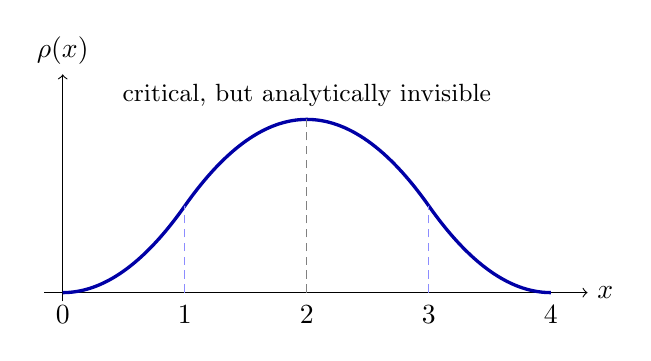
\begin{tikzpicture}[x=1.55cm,y=4.4cm]
 \draw[->] (-.15,0)--(4.3,0) node[right] {$x$};
 \draw[->] (0,-.025)--(0,.63) node[above] {$\rho(x)$};
 \draw[blue!65!black,very thick,domain=0:1,samples=40] plot (\x,{\x*\x/4});
 \draw[blue!65!black,very thick,domain=1:3,samples=65] plot (\x,{(-\x*\x+4*\x-2)/4});
 \draw[blue!65!black,very thick,domain=3:4,samples=40] plot (\x,{(4-\x)*(4-\x)/4});
 \foreach \x in {1,3} {\draw[densely dashed,blue!45] (\x,0)--(\x,.25);}
 \draw[densely dashed,gray] (2,0)--(2,.5);
 \foreach \x in {0,1,2,3,4} {\node[below] at (\x,-.01) {$\x$};}
 \node[above,align=center,font=\small] at (2,.51) {critical, but analytically invisible};
\end{tikzpicture}
\caption{The pushforward density for lengths $(1,1,2)$. The derivative
of order two jumps at $0,1,3,4$, and has no jump at $2$.}
\end{figure}

Here $P(z)=z(z-1)(z-3)(z-4)$, so the minimal differential order is
four. With $h_3(k)=(k+1)(k+2)(k+3)$, the minimal moment recurrence is
\begin{align*}
 &-12h_3(k)m_k+19h_3(k+1)m_{k+1}\\
 &\hspace{18mm}-8h_3(k+2)m_{k+2}+h_3(k+3)m_{k+3}=0.
\end{align*}
The initial values $m_0=1$, $m_1=2$, $m_2=9/2$ follow from the sum
of three uniform variables. For instance, the recurrence at $k=0$
gives $m_3=11$.

\subsection{Complete order classification for three spheres}
For three positive lengths, only the orders $4,6,8$ occur:
\begin{equation}\label{eq:three-full}
 N(a,b,c)=
 \begin{cases}
 4,&(a,b,c)\text{ is proportional, up to permutation, to }
                  (1,1,1)\text{ or }(1,1,2),\\
 6,&\text{otherwise, two lengths are equal or one is the sum of the other two},\\
 8,&\text{otherwise}.
 \end{cases}
\end{equation}
Indeed, positivity means that a collision of distinct subsets can only
come from equal singleton lengths or from a singleton equalling a
disjoint pair. If neither event occurs, all eight sums are distinct.
Exactly two equal lengths, without the exceptional ratios above, leave
six nonzero terms. A relation $a+b=c$ with $a\ne b$ cancels exactly
the two terms at $c$, also leaving six. The exceptional cases were
proved in Proposition~\ref{prop:three-lengths}.

\subsection{Sharpness for every dimension and rational rank}
Choose positive, rationally independent numbers $b_1,\ldots,b_r$ and
take the tuple
\[
 a=(\underbrace{b_1,\ldots,b_1}_{n-r+1\text{ copies}},b_2,\ldots,b_r).
\]
Its numerator is $(e^{b_1t}-1)^{n-r+1}\prod_{j=2}^r(e^{b_jt}-1)$,
and no exponents from different lattice points collide. Therefore
$N(a)=(n-r+2)2^{r-1}$, proving sharpness in the positive symplectic
setting, not merely for abstract Laurent polynomials.

For the fixed manifold $(S^2)^n$, rationally independent lengths give
$N=2^n=\chi((S^2)^n)$, whereas equal lengths give $N=n+1$.
Hence differential order is not a topological invariant of the
underlying manifold. It reflects the arithmetic of the symplectic
parameters and the cancellations in the chosen moment map.

\subsection{Root-system examples and a classical obstruction}
Repeated lengths are not the only way to attain the sharp bound.
Let $a,b>0$ be rationally independent. The following tuples have
rational rank two and attain $N=2n$:
\[
 (a,b),\quad (a,b,a+b),\quad (a,b,a+b,a+2b),
\]
and
\[
 (a,b,a+b,2a+b,3a+b,3a+2b).
\]
Their lattice vectors are the positive-root patterns of
$A_1\times A_1$, $A_2$, $B_2$, and $G_2$.
The alternating Weyl denominator identities, or direct multiplication,
give respectively $4,6,8,12$ surviving monomials. These classical
root-system cancellations are already part of the pure-product
literature \cite{MaltbyRoots}; their role here is to furnish extremal
Hamiltonian examples.

There is a useful limitation on this list, inherited from discrete
tomography. Suppose $r=2$ and the $n$ integer exponent vectors are
pairwise nonparallel. If the support has size $2n$, it consists exactly
of the $2n$ vertices of the Newton polygon. Every coefficient is then
$1$ or $-1$, and the positive and negative supports each have $n$
points. Divisibility by each binomial implies that sums of the signed
coefficients on every line in that direction vanish. Thus the two
supports have the same discrete X-rays in all $n$ directions.
Alpers--Larman's lattice theorem \cite[Theorem 2.2]{AlpersLarman}
implies that equality is impossible for $n=5$ or $n>6$.
Consequently the possible values are exactly $n\in\{2,3,4,6\}$,
with existence supplied by the displayed examples. This is a consequence
of their theorem, not a new classification of lattice switching sets or
of all extremizing configurations.

\section{Scope and further questions}
The symplectic application is to products of spheres with the diagonal
standard circle action. No assertion here classifies general Hamiltonian
circle actions, reconstructs a symplectic manifold from its moment
measure, or extends the sharp arithmetic bound to arbitrary toric
polytopes. In particular, the Euler characteristic alone cannot give
the lower bound in Theorem~\ref{thm:main}.

Three distinctions matter. Rational rank is not the number of visible
levels; rational dependence need not cause a binary subset-sum collision;
and a collision need not cancel its coefficient. The corank-one theorem
resolves all three alternatives in its stated range. For larger relation
spaces, the support bound remains sharp, while a classification of every
equality configuration is not supplied here.

The main additional questions are to classify equality for intermediate
ranks with several independent relations, and to determine which
arithmetic constraints survive for general moment polytopes. These
questions are outside the proved statements. The present contribution
is the sharp rank bound, its collision-sensitive realization as exact
differential complexity, and the complete recurrence divisibility
statement for this family.


\begin{thebibliography}{10}
\raggedright
\bibitem{DH}
J.~J. Duistermaat and G.~J. Heckman,
On the variation in the cohomology of the symplectic form of the reduced
phase space,
\emph{Inventiones Mathematicae} \textbf{69} (1982), 259--268.
\href{https://doi.org/10.1007/BF01399506}{doi:10.1007/BF01399506}.

\bibitem{AB}
M.~F. Atiyah and R. Bott,
The moment map and equivariant cohomology,
\emph{Topology} \textbf{23} (1984), 1--28.
\href{https://doi.org/10.1016/0040-9383(84)90021-1}{doi:10.1016/0040-9383(84)90021-1}.

\bibitem{BoxSplines}
C. de Boor, K. H\"ollig, and S. Riemenschneider,
\emph{Box Splines}, Applied Mathematical Sciences, vol.~98,
Springer, New York, 1993.

\bibitem{Zaslavsky}
T. Zaslavsky,
The slimmest arrangements of hyperplanes. I: Geometric lattices and
projective arrangements,
\emph{Geometriae Dedicata} \textbf{14} (1983), 243--259.
\href{https://doi.org/10.1007/BF00146905}{doi:10.1007/BF00146905}.

\bibitem{MaltbyPTE}
R. Maltby,
Pure product polynomials and the Prouhet--Tarry--Escott problem,
\emph{Mathematics of Computation} \textbf{66} (1997), 1323--1340.
\href{https://doi.org/10.1090/S0025-5718-97-00865-X}{doi:10.1090/S0025-5718-97-00865-X}.

\bibitem{MaltbyRoots}
R. Maltby,
Root systems and the Erd\H{o}s--Szekeres problem,
\emph{Acta Arithmetica} \textbf{81} (1997), 229--245.
\href{https://doi.org/10.4064/aa-81-3-229-245}{doi:10.4064/aa-81-3-229-245}.

\bibitem{AlpersLarman}
A. Alpers and D.~G. Larman,
The smallest sets of points not determined by their X-rays,
\emph{Bulletin of the London Mathematical Society} \textbf{47}
(2015), 171--176.
\href{https://doi.org/10.1112/blms/bdu111}{doi:10.1112/blms/bdu111}.

\bibitem{KeioUnified}
KEIO,
\emph{Global Proof Transfers and Structural Classifications:
Unified Research Manuscript}, unpublished manuscript, 20 October 2026.
Part IX, weighted graphical Jacobi local connections.

\bibitem{KeioVertex}
KEIO,
\emph{Vertex balance: minimal differential equations for traces of
$\beta$-ensembles, Weyl chamber walks and Bessel moments},
unpublished manuscript, October 2026.
Sections 2--3, indicial transfer and dual singular support.
\end{thebibliography}
\end{document}
